\subsection{Implementaci\'on de matriz esparsa.}


Dado el inmenso tama\~no de la Web en general y considerando que el algoritmo de PageRank puede darse para un subconjunto muy grande de esta Web es necesario contemplar los requisitos de espacio f\'isico intr\'insecos a nuestro problema. As\i mismo, visto que trabajamos con matrices esparsas, fue necesario crear un m\'odulo que tome ventaja de esta propiedad, y que de esta manera minimice el espacio requerido.


%yale format init
Una primera aproximaci\'on fue basarnos en el formato Yale para matrices esparsas, el cual cuenta con tres arreglos:
\begin{itemize}
	\item A : valores distintos de cero pertenecientes a la matriz.
	\item IA : indices en A para los primeros valores de cada fila.
	\item JA : n\'umero de columna para cada valor de A.
\end{itemize}

Este formato parec\'ia ahorrar una cantidad considerable de espacio en memoria, pero surg\'ian problemas a medida que aparec\'ian filas que no conten\'ian ning\'un valor distinto de cero, algo que puede suceder tranquilamente. De repente el arreglo IA se volv�a inconsistente y dejaba de tener sentido.
%yale format out


Finalmente decidimos implementar SparseMatrix en base a un vector de listas, donde cada lista representa una fila (puede ser vacia) y cuyos elementos, de existir, son pares <valor,columna>. No s\'olo simplific\'o la implementaci\'on evitando as\'i mismo el absurdo almacenamiento de los valores nulos, sino que tambi\'en mejora el tiempo de ejecuci\'on para la multiplicaci\'on Matriz-Vector, dado que �nicamente se toman en consideraci�n los valores no nulos de cada fila y cada uno viene acompa�ado del \'indice del valor en el vector con el cual de lo debe multiplicar.

\subsection{M\'etodo de la potencia optimizado}

El m\'etodo de la potencia \cite[Secci\'on 9.3]{Burden} es un algoritmo que me permite hallar el m\'aximo autovalor de una matriz, junto a su autovector. La idea principal del m\'etodo es multiplicar un vector sucesivas veces por una matriz. El resultado de realizar esto es que el vector original se transforma seg\'un los autovalores de la matriz y se orienta seg\'un los autovectores de la misma. Si existe un autovalor que es dominante, o sea, es m\'as grande que el resto de los dem\'as, es intuitivo pensar que el vector que es multiplicado se transforme seg\'un ese autovalor y apunte a la direcci\'on de dicho autovector. Ahora, como sabemos que el autovalor dominante de la matriz $P_{2}$ es 1 sabemos que el vector no se va a transformar y lo \'unico que va a suceder es que se va a orientar hacia el autovector asociado al autovalor 1, justamente lo que queremos hallar. Sin embargo, cada iteraci\'on del m\'etodo de la potencia involucra una multiplicaci\'on de matriz con vector y es una operaci\'on costosa en tiempo de procesamiento. Ser\'ia conveniente hallar una forma de reducir ese costo.

Seg\'un Kamvar et al. \cite[Algoritmo 1]{Kamvar2003} para hacer el m\'etodo de la potencia para el sistema $P_{2}x = y$ es equivalente a realizar el siguiente m\'etodo.

\vspace{0.5cm}

\begin{algorithmic}
	\Function{Algoritmo 1}{\textbf{vector} $x$}{ $= y$}
		\State $a = cPx$
		\State $b = ||x||_{1} - ||a||_{1}$
		\State $y = a + bv$
		\State \Return $y$
	\EndFunction
\end{algorithmic}

\vspace{0.5cm}

De modo que el m\'etodo de la potencia queda estructurado de la siguiente manera.

\vspace{0.5cm}

\begin{algorithmic}
	\Function{power method}{}{ $= x^{(n)}$}
		\State \textbf{vector} $x^{(0)} \gets v$
		\State $k \gets 1$ \Repeat
		\State $x^{(k)} \gets \text{Algoritmo 1}(x^{(k-1)})$
		\State $\delta \gets ||x^{(k)} - x^{(k-1)}||_{1}$ \Until $\delta < \epsilon$
		\State \Return $x^{(k)}$
	\EndFunction
\end{algorithmic}

\vspace{0.5cm}

El m\'etodo itera varias veces hasta que la diferencia entre dos iteraciones sucesivas sea menor a un $\epsilon$ dado. Como podemos asegurar convergencia a partir de cualquier $x^{(0)}$ ya que la matriz $P_{2}$ es estoc\'astica por columnas por lo tanto se cumple la proposici\'on 5  exhibida en Bryan \& Leise \cite[Secci\'on 4]{Bryan2006}.

Sin embargo, cada iteraci\'on del m\'etodo de la potencia lleva bastante tiempo, incluso con el Algoritmo 1, as\'i que es necesario tratar de acelerar la convergencia de alguna manera. Esto lo lograremos con el siguiente algoritmo, extrapolaci\'on cuadr\'atica.


\subsection{Extrapolaci\'on cuadr\'atica}

El m\'etodo de extrapolaci\'on cuadr\'atica \cite[Secci\'on 4]{Kamvar2003}consiste en asumir que la matriz $P_{2}$ tiene solo 3 autovectores con 3 autovalores asociados y por lo tanto $x^{(k-3)}$ se puede escribir como combinaci\'on lineal de esos autovectores. Esto nos va a permitir entonces hallar una f\'ormula cerrada para calcular $x^{(k+1)}$ en base a las iteraciones anteriores $x^{(k-3)} \dots x^{(k)}$. Por supuesto, la matriz $P_{2}$ tiene m\'as autovectores que 3 y por lo tanto el valor obtenido es una aproximaci\'on al valor real. Sin embargo, se observa que, a medida que aumenta la cantidad de iteraciones esa aproximaci\'on es bastante buena.

Si suponemos que la matriz tiene solo 3 autovectores $x^{(k-3)}$ se puede escribir como combinaci\'on lineal de esos autovectores:

\[
	x^{(k-3)} = u_{1} + \alpha_{2}u_{2} + \alpha_{3}u_{3}
\]

Luego podemos escribir a las iteraciones sucesivas de la siguiente manera:

\begin{align*}
	x^{(k-2)} &= P_{2}x^{(k-3)}\\
	x^{(k-1)} &= P_{2}x^{(k-2)}\\
	x^{(k)} &= P_{2}x^{(k-1)}
\end{align*}

Luego sea $p$ el polinomio car\'acteristico de $P_{2}$ es un polinomio de grado 3. Las ra\'ices del polinomio son los autovalores de la matriz, en especial el autovalor que conocemos, 1. Evaluando el polinomio en 1 obtenemos:

\[
	p(1) = \gamma_{0} + \gamma_{1} + \gamma_{2} + \gamma_{3} = 0
\]

Luego definamos lo siguiente:

\begin{align*}
	y^{(k-2)} =& x^{(k-2)}- x^{(k-3)} \\
	y^{(k-1)} =& x^{(k-1)}- x^{(k-2)}\\
	y^{(k)} =& x^{(k)}- x^{(k-1)}
\end{align*}

En Kamvar et al.[Secci\'on 5]\cite{Kamvar2003} se utiliza un teorema que me dice que evaluar el polinomio car\'acter\'istico en la matriz $P_{2}$ y multiplicarlo por cualquier vector $z \in \mathbb{R}^{n}$ y el resultado es igual a 0. Adem\'as, sea $z = x^{(k-3)}$, entonces resulta que:

\begin{align*}
	p(P_{2})x^{(k-3)}	=& [\gamma_{0}I + \gamma_{1}P_{2} + \gamma_{2}(P_{2})^{2} + \gamma_{3}(P_{2})^{3}]x^{(k-3)} = 0 \\
						=& \gamma_{0}x^{(k-3)} + \gamma_{1}x^{(k-2)} + \gamma_{2}x^{(k-1)} + \gamma_{3}x^{(k)}= 0 \\
						=& (- \gamma_{1} - \gamma_{2} - \gamma_{3})x^{(k-3)} + \gamma_{1}x^{(k-2)} + \gamma_{2}x^{(k-1)} + \gamma_{3}x^{(k)}= 0 \\
						=& (x^{(k-2)}- x^{(k-3)})\gamma_{1} + (x^{(k-1)}- x^{(k-3)})\gamma_{2} + (x^{(k)}- x^{(k-3)})\gamma_{3}\\
						=& y^{(k-2)}\gamma_{1} + y^{(k-1)}\gamma_{2} + y^{(k)}\gamma_{3}
\end{align*}

Esto se puede escribir en forma matricial de esta manera:

\begin{align}
	\left(y^{(k-2)} \quad  y^{(k-1)} \quad  y^{(k)}\right)\gamma = 0 \label{sistmat}
\end{align}

Como no estamos interesados en la soluci\'on trivial $\gamma = 0$, pediremos que $\gamma_{3} = 1$. Por lo tanto el sistema \eqref{sistmat} puede reescribirse como:

\begin{align}
	\left(y^{(k-2)} \quad y^{(k-1)}\right)\gamma = - y^{(k)} \label{sistmat2}
\end{align}

Resolviendo ese sistema hallamos los valores de $\gamma$(veremos m\'as adelante como realizaremos este paso) y por lo tanto los coeficientes del polinomio $p$. Ahora, sea $q$ un polinomio definido de la siguiente manera:

\begin{align}
	q(\lambda) = \frac{p(\lambda)}{(1-\lambda)} = \beta_{0} + \beta_{1}\lambda + \beta_{2}\lambda^{2} \label{polq}
\end{align}

Como ya sabemos los valores de $\gamma$ podemos despejar los valores de $\beta_{i}$ de manera que:

\begin{align*}
	\beta_{0} &= \gamma_{1} + \gamma_{2} + \gamma_{3} \\
	\beta_{1} &= \gamma_{2} + \gamma_{3} \\
	\beta_{2} &= \gamma_{3}
\end{align*}

Nuevamente por el teorema utilizado anteriormente vale que para cualquier vector $r$:

\[
	q(P_{2})r = u_{1}
\]

Sea $r = x^{(k-2)}$ entonces vale la siguiente igualdad

\begin{align*}
	q(P_{2})x^{(k-2)} =& [\beta_{0}I + \beta_{1}P_{2} + \beta_{2}(P_{2})^{2}]x^{(k-2)}\\
	u_{1} =& \beta_{0}x^{(k-2)} + \beta_{1}x^{(k-1)} + \beta_{2}x^{(k)}
\end{align*}

Y eso es justamente lo que quer\'iamos obtener. Por lo tanto tenemos una nueva aproximaci\'on a $u_{1}$ basado en valores anteriores de la sucesi\'on $\{x^{(n)}\}$.

Nos queda por decidir como resolver el sistema planteado en \eqref{sistmat2} de forma eficiente de manera que realizar extrapolaci\'on quadr\'atica no sea costosa. Definimos lo siguiente:

\[
	Y = \left(y^{(k-2)} \quad y^{(k-1)}\right)
\]


Se observa que $Y$ es un sistema sobredeterminado ya que hay m\'as filas que columnas, por lo tanto la soluci\'on obtenida es aquella de resolver el problema de cuadrados m\'inimos. Una forma de encontrar la soluci\'on de cuadrados m\'inimos es utilizando la factorizaci\'on QR. Dicha factorizaci\'on consiste en poder descomponer la matriz $Y \in \mathbb{R}^{n \times 2}$ en el producto de dos matrices: $Q\in \mathbb{R}^{n \times n}$ y $R\in \mathbb{R}^{n \times 2}$, de manera que:

\begin{align*}
	Y\gamma &=-y^{(k)}\\
	QR\gamma &=-y^{(k)}\\
	R\gamma &=-Q^{t}y^{(k)}\\
\end{align*}

\begin{figure}[!h]
	\begin{center}
		  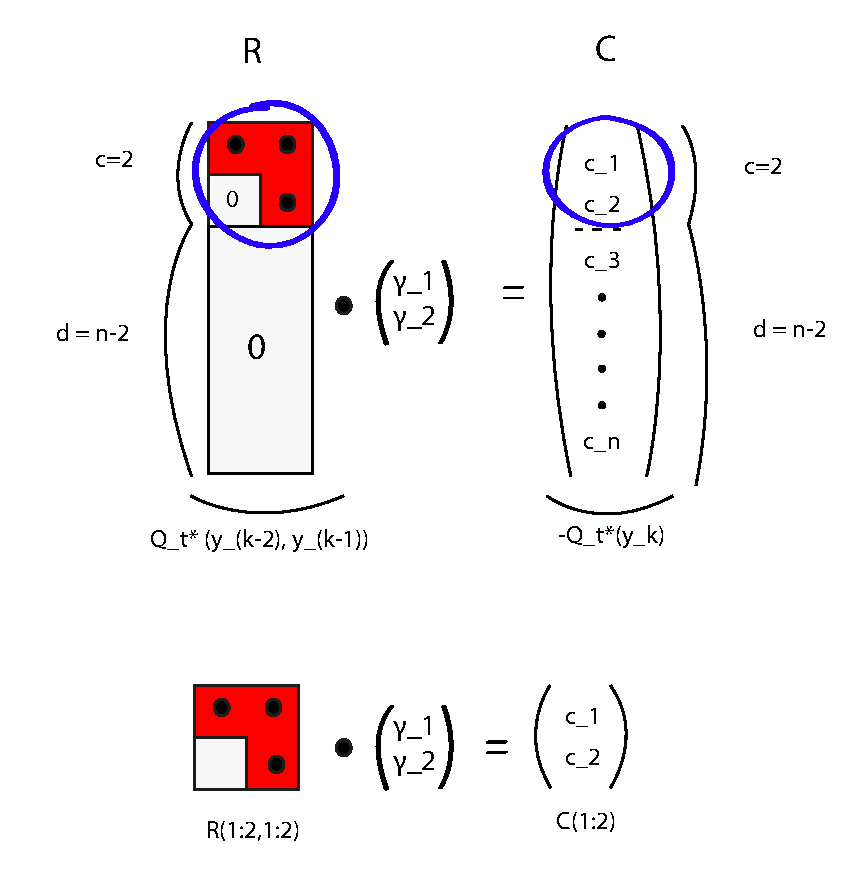
\includegraphics[scale = 0.5]{graficos/im_1.pdf}
		  \caption{Sistema a resolver simplificado}
		  \label{fig:contra1}
	\end{center}
\end{figure}
\FloatBarrier
Y esto resulta un sistema f\'acil para resolver utilizando \emph{backwards-substitution}.

Uno de los m\'etodos vistos en la materia para obtener la factorizaci\'on QR fue el m\'etodo de \emph{Householder} \cite{Burden} que me permite reflejar ortogonalmente las columnas de $Y$ y as\'i ir obteniendo la matriz triangular superior $R$. Se puede observar que como la matriz $Y$ tiene solo 2 columnas entonces en 2 pasos de \emph{Householder} se obtiene la $R$ deseada. El problema es la dimensi\'on de $Q$. Al ser $n$ muy grande (que es lo esperado), calcularla en base al producto de $Q_1$ (primer paso de \emph{Householder}) y $Q_2$ (segundo paso de \emph{Householder}) es muy costoso en cuanto a recursos de memoria. Con \emph{web-Stanford} como entrada, la factorizaci\'on $QR$ cuelga el sistema ya que se queda sin memoria. 

Es por esto que implementamos \emph{Householder eficiente}, donde buscamos obtener $R$ y $-Q^{t}y^{(k)}$ a trav\'es de sucesivas multiplicaciones del tipo Matriz-Vector, y resta de matrices. Evitar el almacenamiento en memoria y producto de matrices de $n \times n$ es importantisimo en el contexto de este trabajo, ya que hablamos de un \'orden de $O(n^3)$ para el producto y $O(2*n^2)$ en memoria.

A continuaci\'on, el primer paso de \emph{Householder eficiente}. El segundo es an\'alogo.

~

$(I - 2uu^{t})*A = (I - 2uu^{t})*b$

$(A - 2uu^{t}A) = (b - 2uu^{t}b)$

~

Notemos que $u^{t}*b$ es un escalar (por lo que simplifica mucho las operaciones). Además no tenemos que multiplicar por la 
identidad ya que el paso resulta trivial.

Volviendo al problema de hallar $P_{2}x = y$, el algoritmo con la optimización es entonces: 

~

\begin{algorithmic}
	\Function{power method with quadratic extrapolation}{}{ $= x^{(n)}$}
		\State \textbf{vector} $x^{(0)} \gets v$
		\State $k \gets 1$ \Repeat
		\State $x_{k-3} \gets x_{k-2}$
		\State $x_{k-2} \gets x_{k-1}$
		\State $x_{k-1} \gets x_{k}$
		\State $x^{(k)} \gets \text{Algoritmo 1}(x^{(k-1)})$
		\If{someConditionAboutk}
			\State $x^{(k)} \gets$ QuadraticExtrapolation($x_{k-3},x_{k-2},x_{k-1},x_{k}$)
		\EndIf
		\State $\delta \gets ||x^{(k)} - x^{(k-1)}||_{1}$ \Until $\delta < \epsilon$
		\State \Return $x^{(k)}$
	\EndFunction
\end{algorithmic}



